\section{An Example}
Consider the following input graph drawing $\Gamma_G$:
\begin{figure}[H]
	\centering
	\begin{subfigure}{\textwidth}
		\centering
		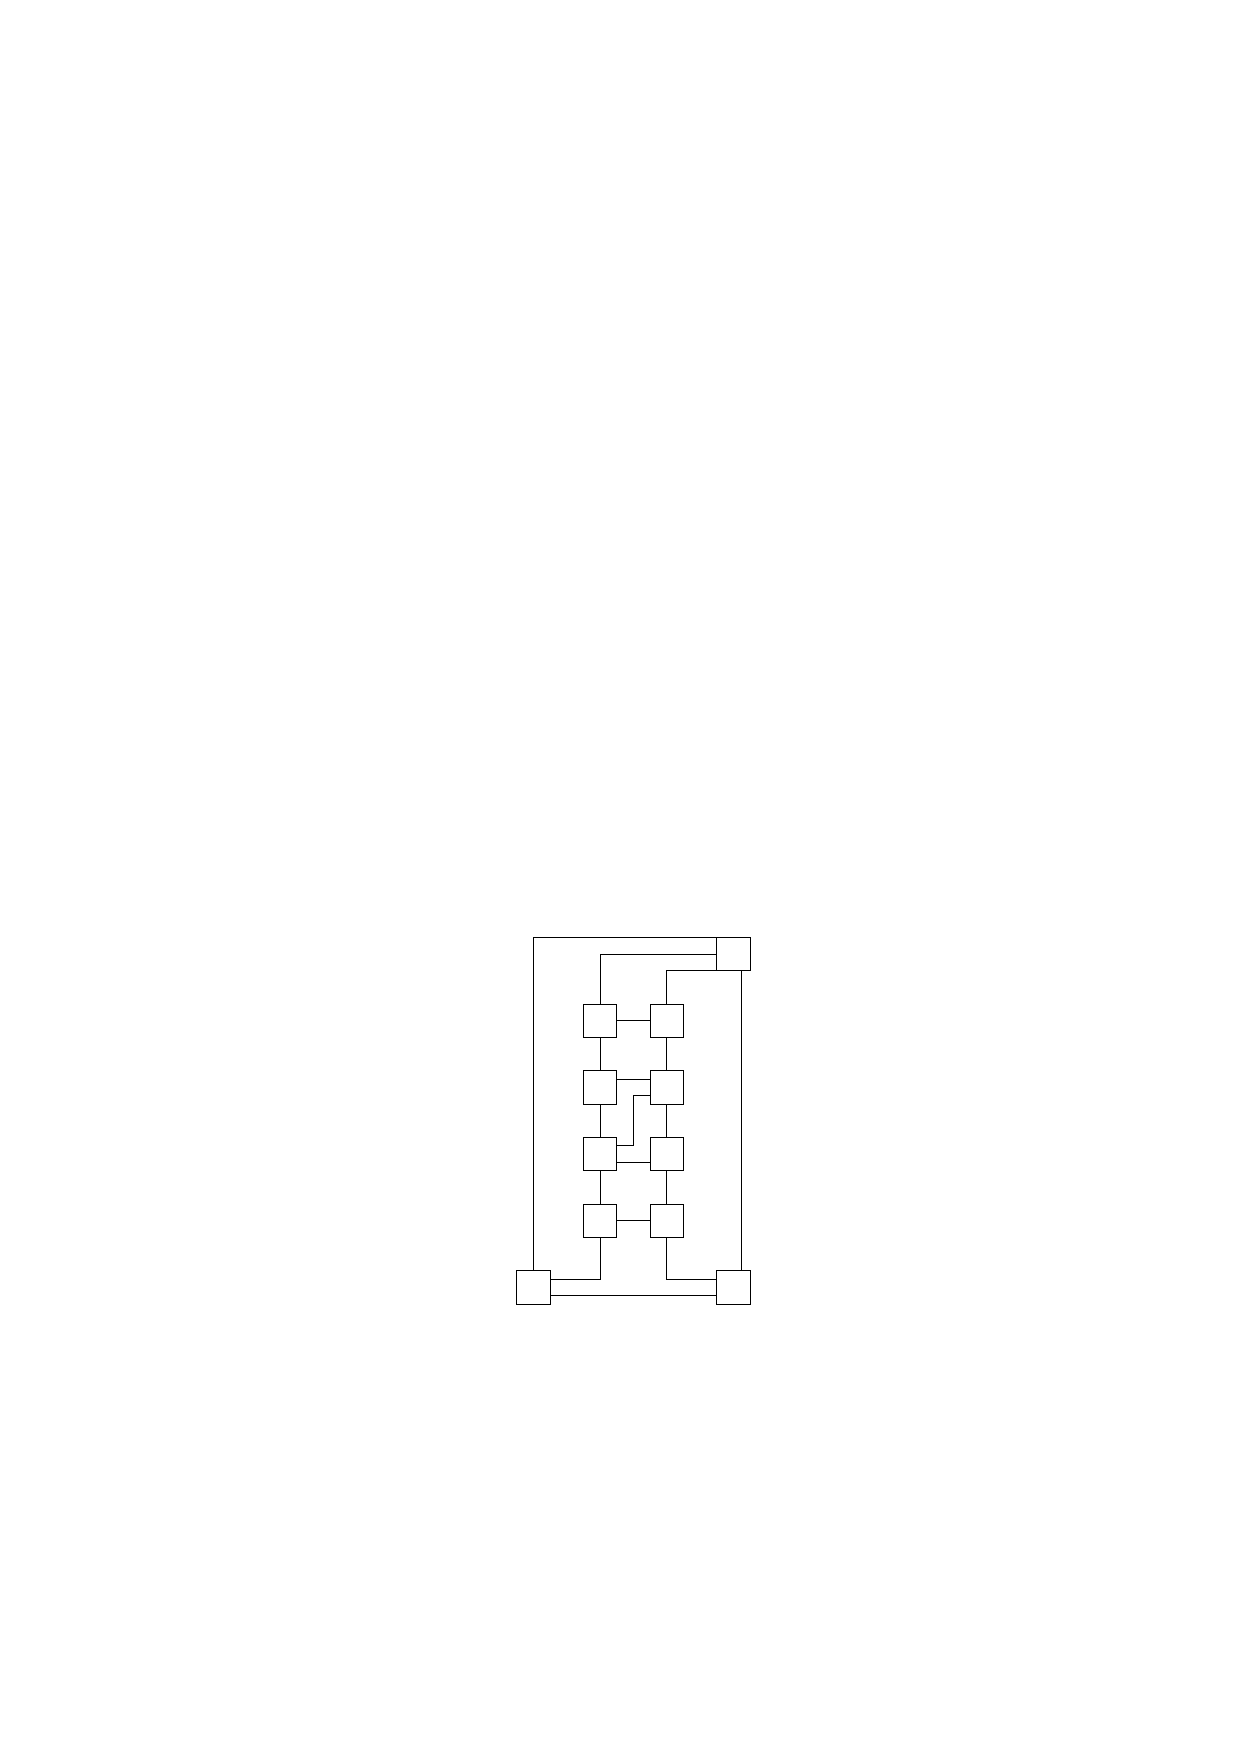
\includegraphics[width=0.2\linewidth,page=1]{includegraphics/big-example}
	\end{subfigure}
	\caption{Example input drawing $\Gamma_G$}
\end{figure}
For measurement, the unit of length lies in the width of the illustrated boxes. The longest vertical segment lies on the left of the drawing and is of length 10. The complexity of the drawing equals three. The drawing is of size $7\times11$. 
\begin{figure}[H]
	\centering
	\begin{subfigure}{\textwidth}
		\centering
		\includegraphics[width=0.8\linewidth,page=2]{includegraphics/big-example}
	\end{subfigure}
	\caption{$\Gamma_G$ after the stretching technique application}
\end{figure}
\begin{figure}[H]
	\centering
	\begin{subfigure}{\textwidth}
		\centering
		\includegraphics[width=0.8\linewidth,page=3]{includegraphics/big-example}
	\end{subfigure}
	\caption{$\Gamma_G$ after the circular arc substitution}
\end{figure}
After stretching and smoothening the complexity of the resulting SMOG drawing rises from 3 to $\left\lfloor\frac{3}{2}\cdot 3\right\rfloor = 4$. The size of the drawing equals $37\times11$. The drawing inherits some redundancy which we can get rid of thanks to the saving measures.
\begin{figure}[H]
	\centering
	\begin{subfigure}{\textwidth}
		\centering
		\includegraphics[width=0.6\linewidth,page=4]{includegraphics/big-example}
	\end{subfigure}
	\caption{$\Gamma_G$ after the saving plane sweep application}
\end{figure}
The drawing lost 51,4\% in horizontal area requirements resulting in a drawing with $18\times11$ area bounds. Also, the complexity decreased from 4 to 3.
\begin{figure}[H]
	\centering
	\begin{subfigure}{\textwidth}
		\centering
		\includegraphics[width=0.6\linewidth,page=7]{includegraphics/big-example}
	\end{subfigure}
	\caption{$\Gamma_G$ after the port reassignment}
\end{figure}
The port reassignment results in a smoothened drawing of complexity 2 and the area consumption can further be reduced, resulting in a drawing of size $16\times 11$.